%!TEX root = paper.tex
\chapter{A tutorial of \Backpack{}}
\label{sec:tour}

In this section, we will walk through a tutorial of taking a Haskell'98
regular expression matcher taken
from~\cite{Fischer:2010:PRE:1863543.1863594}, highlighting the main
features of \Backpack{} as well as introducing some core conceptual
ideas which will be elaborated upon later in this thesis.  We'll assume
familiarity with Haskell'98 or an ML-like language, but won't assume you
know anything about Cabal (Haskell's package management system) or
\OldBackpack{}~\cite{backpack}.

\section{A simple matcher in '98}

In Figure~\ref{fig:matcher-haskell98}, we reproduce the source code of
the simple, inefficient regular expression matcher
from~\cite{Fischer:2010:PRE:1863543.1863594} and a small test program.
We'll use this code to briefly describe how Haskell's existing module
and package system works; experienced readers should feel free to skip
ahead to the next section.

\begin{figure}
\begin{lstlisting}
module Regex (Reg(..), accept) where

-- | A type of regular expressions.
data Reg = Eps | Sym Char | Alt Reg Reg | Seq Reg Reg | Rep Reg

-- | Check if a regular expression 'Reg' matches a 'String'
accept :: Reg -> String -> Bool
accept Eps       u = null u
accept (Sym c)   u = u == [c]
accept (Alt p q) u = accept p u || accept q u
accept (Seq p q) u = or [accept p u1 && accept q u2 | (u1, u2) <- splits u]
accept (Rep r)   u = or [and [accept r ui | ui <- ps] | ps <- parts u]

-- | Compute all splits of the string.
splits :: String -> [(String, String)]
splits [] = [([], [])]
splits (c:cs) = ([], c:cs):[(c:s1,s2) | (s1,s2) <- splits cs]

-- | Compute all possible non-empty partitions of the string
parts :: String -> [[String]]
parts [] = [[]]
parts [c] = [[[c]]]
parts (c:cs) = concat [[(c:p):ps, [c]:p:ps] | p:ps <- parts cs]
\end{lstlisting}
\caption{Source code for a regular expression matcher from~\cite{Fischer:2010:PRE:1863543.1863594}.}
\begin{lstlisting}
module Main where

import Regex

nocs = Rep (Alt (Sym 'a') (Sym 'b'))
onec = Seq nocs (Sym 'c')
evencs = Seq (Rep (Seq onec onec)) nocs
main = print (accept evencs "acc")
\end{lstlisting}
\caption{Simple test program for the matcher.}
\label{fig:matcher-haskell98}
\end{figure}

Looking at the source code, we can observe a few things:

\begin{itemize}
    \item The code is organized into two \emph{modules}, each heralded
    by the \verb|module| keyword.  Each module defines types and values
    within a distinct namespace.  Haskell modules are used purely for
    namespacing and do not support any sort of hierarchical organization.

    \item The \verb|import| keyword is used to bring declarations into
    scope from other modules; for example, \verb|Main| imports \verb|Regex|
    to bring the constructors of \verb|Reg| and \verb|accept| into scope.
    Every module also implicitly has an import of \verb|Prelude|, which
    provides many commonly used types and functions (e.g., \verb|print|,
    \verb|String|, etc).

    \item The \verb|Regex| module comes with an \emph{export list}
    \verb|Reg(..), accept)|, which designates which declarations should
    be brought into scope when this module is imported.  The ability to
    omit declarations from an export list (e.g., \verb|splits| and \verb|parts|)
    is one of the primary mechanism by which data abstraction is achieved in
    Haskell: internal implementation details are not exported and thus
    cannot be accessed by end users.
\end{itemize}
Modules themselves are organized into packages, which are described by
\emph{Cabal files}.  For example, the modules above might be organized into
packages with the Cabal files as shown in Figure~\ref{fig:matcher-packages}.
Each package description describes:

\begin{figure}
\begin{tabular}{p{0.45\textwidth} p{0.45\textwidth}}
\begin{lstlisting}[language=Cabal]
-- regex.cabal
name: regex
version: 1.0
library
    exposed-modules: Regex
    build-depends: base
\end{lstlisting}
&
\begin{lstlisting}[language=Cabal]
-- regex-program.cabal
name: regex-program
version: 1.0
executable regex-program
    main-is: Main.hs
    build-depends: base, regex
\end{lstlisting}
\end{tabular}
\caption{Cabal files for the regex and regex-program packages. The Haskell source code
of these packages is in Figure~\ref{fig:matcher-haskell98}.}
\label{fig:matcher-packages}
\end{figure}

\begin{itemize}
    \item The name of the package (\verb|name|),
    \item The version of a package (\verb|version|),
    \item One or more \emph{components} (libraries, executables,
    test-suites, etc.), each of which defines some modules
    (\verb|exposed-modules| and \verb|main-is|) and specifies
    dependencies on other packages (\verb|build-depends|).
    A library exposes modules for other packages to use when
    they \verb|build-depends| on the library, while an
    executable is associated with a particular \verb|hs| file
    which is expected to define a \verb|main| function that
    will serve as the top-level entry of the program.\footnote{For the
    sake of realism, each package above includes \texttt{base} in their
    \texttt{build-depends}, to ensure that the implicitly imported
    \texttt{Prelude} module is in scope.}
\end{itemize}
Packages serve as the unit of distribution: a set of modules organized
into a package can be uploaded to a package repository (e.g., Hackage)
to be shared with other developers.  A \emph{package
manager} (e.g., cabal-install) automates the process of downloading the source code of all
packages one depends upon and building them in order.

\section{Functorizing the matcher}

One problem with the code in Figure~\ref{fig:matcher-haskell98} is that
it only works with \verb|String|s (i.e., \verb|[Char]|).  One easy
generalization (seen in the original
paper~\cite{Fischer:2010:PRE:1863543.1863594}) is to add a type
parameter to \verb|Reg|, so that \verb|accept| operates on lists of
arbitrary symbols rather than just characters.  But this is still not as
general as the matcher could be; for example,
\verb|ByteString| is not a list but a packed array of bytes; here,
we also need to be parametric in the string type itself.

In this case, we can use \Backpack{} to functorize our matcher over an
arbitrary string and element type.  To do this, we create a new
signature named \verb|Str|, which provides abstract string and element
types, and all operations our matcher needs to have supported for it.
The resulting signature and module can be seen in
Figure~\ref{fig:matcher-regex-indef-source}, alongside a module which
implements the string signature.

\begin{figure}
\begin{lstlisting}
signature Str where

data Str
data Chr
instance Eq Str

null      :: Str -> Bool
singleton :: Chr -> Str
splits    :: Str -> [(Str, Str)]
parts     :: Str -> [[Str]]
\end{lstlisting}
\caption{Source code for a signature specifying abstract strings.}

\begin{lstlisting}
module Regex where

import Prelude hiding (null)
import Str

data Reg = Eps | Sym Chr | Alt Reg Reg | Seq Reg Reg | Rep Reg

accept :: Reg -> Str -> Bool
accept Eps       u = null u
accept (Sym c)   u = u == singleton c
accept (Alt p q) u = accept p u || accept q u
accept (Seq p q) u = or [accept p u1 && accept q u2 | (u1, u2) <- splits u]
accept (Rep r)   u = or [and [accept r ui | ui <- ps] | ps <- parts u]
\end{lstlisting}
\caption{Source code for regular expression matcher, parametrized by the Str signature.}
\label{fig:matcher-regex-indef-source}
\end{figure}

Because the original source code of the matcher was not written with
this functorization in mind, the \verb|Regex| had to be modestly
refactored to treat \verb|Str| abstractly.  This included replacing the
use of list operations \verb|null| and \verb|[c]| with abstract
functions, as well as deleting the implementations of \verb|splits| and
\verb|parts|, deferring them to the signature implementation.  However,
no invasive changes---e.g., adding new type parameters or passing new
arguments---were necessary.  The new Cabal file for this signature and
module, seen in Figure~\ref{fig:matcher-regex-indef-cabal}, needs only
to declare \verb|Str| in the \verb|signatures| field.

\begin{figure}
\begin{lstlisting}[language=Cabal]
name: regex-indef
version: 1.0
library
    exposed-modules: Regex
    signatures: Str
    build-depends: base
\end{lstlisting}
\caption{Cabal files for the regex-indef package, which provides a Regex
module parametrized by string implementation.}
\label{fig:matcher-regex-indef-cabal}
\end{figure}

The new \verb|regex-indef| package can be typechecked, even though no
implementation of \verb|Str| is provided (as one would expect under
separate modular development).

\section{An implementation of Str}

Before we instantiate \verb|regex-indef|, we will need an implementation
of the \verb|Str| signature.  Figure~\ref{fig:matcher-str-string-source}
provides one such implementation.

\begin{figure}
\begin{tabular}{p{0.55\textwidth} p{0.40\textwidth}}
\begin{lstlisting}
module Str.String where

import Prelude as P

type Str = String
type Chr = Char

null   = P.null :: Str -> Bool
singleton = (\c -> [c]) :: Chr -> Str
splits = ... :: Str -> [(Str, Str)]
parts  = ... :: Str -> [[Str]]
\end{lstlisting}
&
\begin{lstlisting}[language=Cabal]
name: str-string
version: 1.0
library
    exposed-modules: Str.String
    build-depends: base
\end{lstlisting}
\end{tabular}
\caption{An implementation of Str, alongside its package description.}
\label{fig:matcher-str-string-source}
\end{figure}

The \verb|...| is a placeholder for the implementations \verb|splits|
and \verb|parts| from Figure~\ref{fig:matcher-haskell98}. One thing to
note is that we must declare \verb|null| and \verb|singleton| with
explicit type signatures, as signature matching in Haskell requires two
declarations to have exactly the same type: the polymorphic function
\verb|[a] -> Bool| is not considered a valid implementation of
\verb|[Char] -> Bool|.  Signatures in Backpack are width-subtyped, so
\verb|Str.String| could also contain more exported functions, and still
be considered to implement \verb|Str|.

%   In practice, the current convention in the Haskell community when
%   defining new modules is to pick a new name.  Thus, it's more likely
%   that the \verb|Str| module from \verb|str-string| will actually
%   be named something like \verb|Str.String|.  In this case,

\section{Instantiating the matcher}

How do we actually go about instantiating our matcher with the
implementation of Str from Figure~\ref{fig:matcher-str-string-source}?
In a traditional, ML module system, there would be a module language for
expressing how to instantiate a functor.
In \Backpack{}, a client instantiates a package by bringing its
requirements into scope with another module under the same name.  A
module and signature with the same name are \emph{mix-in linked}
together.  For example, the executable \verb|regex-program| uses the
\verb|mixins| field to rename the module from \verb|str-string| to the
same name as \verb|regex-indef|'s signature.%
%
\footnote{Why didn't \texttt{str-string} just export
a module named \texttt{Str}?  The prevailing convention in the Haskell
community is that modules should be given unique names; naming all
implementations of the \texttt{Str} signature \texttt{Str} would violate
this convention.  At this point in time, it's not clear if the
convenience of not needing to rename modules overrides the benefits of
being able to refer to a module uniquely by its name.}

\begin{figure}
\begin{lstlisting}[language=Cabal]
name: regex-program
version: 1.0
executable regex-program
    main-is: Main.hs
    build-depends: base, regex-indef, str-string
    mixins: str-string (Str.String as Str)
\end{lstlisting}
\caption{Package descriptions for \texttt{regex-program}, which brings
Regex into scope instantiated with the \texttt{Str} implementation from \texttt{str-string}.}
\label{fig:matcher-functorized-packages}
\end{figure}

What actually happens when mix-in linking takes place?  There are two very useful
ways to understand the process.  First, in Figure~\ref{fig:regex-indef-instantiated}, we
\emph{pictorially} represent each depended upon library as a block, with input and output
ports representing signatures and modules respectively.  Intuitively, the process
of mix-in linking involves ``wiring up'' these signatures and modules based on the
names they have been ascribed.

\begin{figure}
\center%
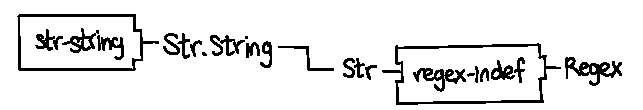
\includegraphics{figures/regex-indef-instantiated.pdf}
\caption{This is the wiring diagram for regex-program. The left side of blocks
(representing libraries) have input ports (required signatures), while the right hand side
of blocks have output ports (provided modules). Ports are wired to show how requirements are
filled: a kink indicates some renaming took place. Mixin linking wires up requirements
and provisions which have the same module name.}
\label{fig:regex-indef-instantiated}
\end{figure}

Second, we can consider an intermediate representation of the package language
\emph{after} mix-in linking,
as in Figure~\ref{fig:matcher-bkp}, where every dependency on another library
is given an \emph{explicit instantiation} specifying how all of its requirements
are filled; we will call this the \emph{syntactic} interpretation of
the package description. The name of the library plus an instantiation is referred
to as a \emph{\uid{}}.  In the case of \verb|regex-indef|, the
\uid{} indicates that the requirement \verb|Str| is to be filled
with the module \verb|Str.String| from the library \verb|str-string|.\footnote{In
fact, GHC 8.2 comes with a mode for directly parsing and compiling this intermediate
representation, which is used extensively by our test suite.}  This intermediate
representation will play an important role in managing the abstraction barrier
between the compiler and package manager, and we will repeatedly return to
it throughout the rest of this thesis.

\begin{figure}
\begin{lstlisting}
unit regex-program where
    dependency base
    dependency str-string
    dependency regex-indef[Str=str-string:Str.String]
    module Main where ...
\end{lstlisting}
\caption{The intermediate representation of the packages from Figure~\ref{fig:matcher-functorized-packages}.
The reference to \texttt{regex-indef} in \texttt{regex-program} now consists of an explicit functor application.}
\label{fig:matcher-bkp}
\end{figure}

One important practical consideration is whether or not there is any
performance cost to using signatures, deferring the implementation of
a module until later.  In particular, if one separately
compiles uninstantiated components to machine code, no cross-package
inlining can occur, since the component is compiled only against a
signature and not against the code that implements the signature.  For
Haskell and GHC, cross-module inlining is a major contributor to
performance, so our implementation of \Backpack{} does \emph{not}
separately compile uninstantiated packages. Instead, every distinct
instantiation of a component is compiled against the code that
implements its requirements. This process is managed by Cabal to avoid
unnecessary recompilation, similarly to how Cabal avoids recompiling
dependencies that are already installed.

\section{Reusing libraries with different instantiations}

The reason we parametrized \verb|regex| was so that we could use it
with another implementation of \verb|Str|.  Figure~\ref{fig:str-bytestring}
gives a \verb|bytestring| based implementation of \verb|Str|, which shows
off another aspect of signature matching with Backpack: declarations from
a signature do not have to be implemented by the module itself: they can
be \emph{reexported} from another module.  In this example, all the declarations
defined in \verb|Data.ByteString|, which include \verb|null| and \verb|singleton|,
are reexported by the \verb|module Data.ByteString| line in the export list
of \verb|Str.ByteString|.

\begin{figure}
\begin{lstlisting}
module Str.ByteString (
    module Data.ByteString,
    Str, Chr,
    splits, parts,
) where

import Prelude hiding (length, null, splitAt)
import Data.Word
import Data.ByteString

type Str = ByteString
type Chr = Word8

splits :: Str -> [(Str, Str)]
splits s = fmap (\n -> splitAt n s) [0..length s]

parts :: Str -> [[Str]]
parts s | null s    = [[]]
        | otherwise = do n <- [1..length s]
                         let (l, r) = splitAt n s
                         fmap (l:) (parts r)
\end{lstlisting}
\begin{lstlisting}[language=Cabal]
name: str-bytestring
version: 1.0
library
    exposed-modules: Str.ByteString
    build-depends: base, bytestring
\end{lstlisting}
\caption{An implementation of Str backed by \texttt{bytestring},
and its package description.}
\label{fig:str-bytestring}
\end{figure}

We can modify \verb|regex-program| to use \verb|str-bytestring| instead
of \verb|str-string| when instantiating \verb|regex-indef| by modifying
all appropriate references in the Cabal file.  However, we can also use
both instantiations at the same time by specifying \verb|regex-indef|
twice in \verb|mixins|, as seen in the Cabal file in
Figure~\ref{fig:regex-program-multi}.

\begin{figure}
\begin{lstlisting}[language=Cabal]
name: regex-program
version: 1.0
executable regex-program
    main-is: Main.hs
    build-depends: base, regex-indef, str-string, str-bytestring
    mixins:
        regex-indef (Regex as Regex.String) requires (Str as Str.String),
        regex-indef (Regex as Regex.ByteString) requires (Str as Str.ByteString)
\end{lstlisting}
\caption{Package descriptions for \texttt{regex-program}, which brings
Regex into scope instantiated with the \texttt{Str} implementation from \texttt{str-string}.}
\label{fig:regex-program-multi}
\end{figure}

Instead of renaming the module from \verb|str-string| to be \verb|Str|,
we instead rename the \emph{requirement} from \verb|regex-indef| to
\verb|Str.String| and \verb|Str.ByteString|.  This gives us two copies
of \verb|regex-indef|: one with \verb|Str| filled with
\verb|Str.String|, and the other with \verb|Str| filled with
\verb|Str.ByteString|.  To distinguish the provided modules of each
instance, we rename them to two distinct names which \verb|Main|
can import independently.  We can visualize these two instantiations
diagramatically, as in Figure~\ref{fig:regex-indef-twice}, or
we can look at the intermediate representation of the package language
after mixin linking, as in Figure~\ref{fig:matcher-twice-bkp}.

\begin{figure}
\center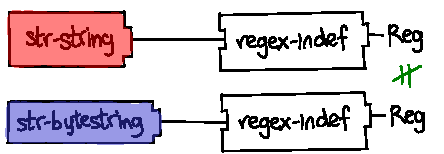
\includegraphics{figures/regex-indef-twice.pdf}
\caption{Two instantiations of \texttt{regex-indef} which each define
\texttt{Reg}.  These \texttt{Reg}s are not type equivalent, because
their respective wiring diagrams are different.}
\label{fig:regex-indef-twice}
\end{figure}

\begin{figure}
\begin{lstlisting}
unit regex-program where
    dependency base
    dependency str-string
    dependency str-bytestring
    dependency regex-indef[Str=str-string:Str.String] (Regex as Regex.String)
    dependency regex-indef[Str=str-bytestring:Str.ByteString] (Regex as Regex.ByteString)
    module Main where
        import qualified Regex.String
        import qualified Regex.ByteString
        ...
\end{lstlisting}
\caption{The intermediate representation \texttt{regex-program} with two instantiations of \texttt{regex-indef}.  The \uid{}s after \texttt{dependency} form the type identity of the entities declared in \texttt{Regex.String} and \texttt{Regex.ByteString}.}
\label{fig:matcher-twice-bkp}
\end{figure}

An important subtlety arises in this situation.  Ordinarily, two types
are considered equivalent if they have the same \emph{identity}: an
identity consists of both the name of the type and the name of the
module which originally defined the type.  Consider the \verb|Reg| type,
which refers to \verb|Chr|: the identity of \verb|Reg| must somehow
depend on how we decided to implement \verb|Chr|: a \verb|Reg|
containing a \verb|Char| is very different from a \verb|Reg| containing
a \verb|Word8|.

In fact, \Backpack{} takes a conservative approach to determining the
identity of a type: it computes the type identities of all identifiers
defined in a package based on the identities of the modules that fill
the signatures of the package.  Diagramatically, the identity
incorporates the \emph{wiring diagrams} of the components which defined
the types in question; in the intermediate representation after mix-in
linking, the identity incorporates the \uid{} (which
identifies both the library and how it is instantiated.)

\section{Composing libraries with requirements}

When we discussed instantiation, we stated that modules and signatures
with the same name would be linked together.  If two signatures from the
same library are brought into scope under the same name, they will also
be linked, effectively \emph{merging} the two requirements together.
For example, suppose that you had two packages \verb|p| and \verb|q|
which both were parametrized by \verb|Str|, with the first and second
signatures in Figure~\ref{fig:signature-merging}.  If we were to use
both packages together in the same third package \verb|r| (e.g.,
\verb|build-depends: p, q|), the two \verb|Str| signatures would merge
to form the third signature in Figure~\ref{fig:signature-merging}.

\begin{figure}
\begin{tabular}{p{0.30\textwidth} p{0.30\textwidth} p{0.30\textwidth}}
\begin{lstlisting}
signature Str where
  data Str
  null  :: Str -> Bool
\end{lstlisting}
&
\begin{lstlisting}
signature Str where
  data Str

  empty :: Str
\end{lstlisting}
&
\begin{lstlisting}
signature Str where
  data Str
  null  :: Str -> Bool
  empty :: Str
\end{lstlisting}
\end{tabular}
\caption{The first and second signatures merge to form the third signature.}
\label{fig:signature-merging}
\end{figure}

As before, Figure~\ref{fig:signature-merging-interp} illustrates the
pictorial and syntactic interpretations of this merging process.  It's
worth pointing out that in the syntactic interpretation, the first
occurrence of \verb|<Str>| is a binding occurrence for the subsequent
occurrences of \verb|<Str>| in the body of the unit.  The implementation
of \verb|Str| for \verb|r| ``flows'' to also implement the requirements
of \verb|p| and \verb|q|; conversely, the specific required entities
from the signatures of \verb|p| and \verb|q| flow back to form \verb|r|'s
merged requirement.%
%
\footnote{In the package description, it's not necessary to declare \texttt{Str}
in the \texttt{signatures} field, as it can be inferred from the requirements
of \texttt{p} and \texttt{q}.  We render it explicitly in the intermediate
representation for clarity.}

\begin{figure}
\begin{tabular}{p{0.45\textwidth} p{0.45\textwidth}}
\center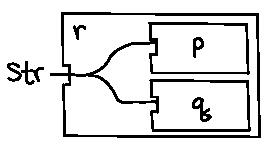
\includegraphics{figures/p-q-merge-Str.pdf}
&
\vspace{2em}
\begin{lstlisting}
unit r <Str> where
    dependency p[Str=<Str>]
    dependency q[Str=<Str>]
\end{lstlisting}
\end{tabular}
\caption{Representation of \texttt{r} as a diagram, and as the intermediate
representation after mix-in linking.}
\label{fig:signature-merging-interp}
\end{figure}

Libraries with requirements can be composed in arbitrarily complex ways;
for example, a requirement can be filled with a module from another library,
which itself has a requirement.  Because type identity relies
only on how a package is instantiated (and not when it is instantiated),
it makes no difference to the end user whether or not a library
is instantiated earlier or later.

\section{Refining types in signatures}

Suppose that you wanted to write a library of regular expressions for
matching, say, e-mails, which you wanted to build atop of
\texttt{regex-indef}.  In particular, you want to keep the particular
\emph{string} representation (\verb|Str|) abstract, but you want
to assert that, whatever string it is, it consists of Unicode
characters (\verb|Char|).  With ML modules, you would have to take
advantage of another feature such as ``destructive substitution''
to apply this assertion to an existing signature.  In \Backpack{}, you
write a small signature to link with the existing signature:

\begin{lstlisting}
    signature Str where
        type Chr = Char
\end{lstlisting}

\noindent
The effect of linking this signature to \verb|regex-indef| is that
all occurrences of \verb|Chr| are all refined to be \verb|Char|;
for example, with this signature you can now write the regular
expressions (e.g., \verb|Rep (Alt (Sym 'a') (Sym 'b'))|) from
\verb|regex-program| or pass a \verb|Char| to \verb|singleton|.
Previously, this would not have been possible, because the
abstract type \verb|Chr| was considered distinct from \verb|Char|.

\section{Reusing and thinning signatures}

For applications more complex than a regular expression matcher, the set
of operations one might need from a string implementation will expand
correspondingly.  In such a case, there will be less code duplication if
a signature for strings is written once and then reused packages that
need it.

A signature can be straightforwardly packaged into a library, simply
by declaring a library with one or more signatures, but no modules.
We call such packages \emph{signature packages}:

\begin{lstlisting}[language=Cabal]
    name: str-sig
    version: 1.0
    library
        signatures: Str
        build-depends: base
\end{lstlisting}

\noindent
In fact, \Backpack{} treats such signature packages specially.
Ordinarily, a required signatures cannot be thinned: if you are using a
package that requires \verb|null :: Str -> Bool|, you must \emph{always}
provide that entity (since it may be used to implement some provided
function which you are making use of).  However, this is never the case
for a signature package; an entity declared in a signature here is only
ever used in the types of another package.  So \Backpack{} permits you
to thin requirements of signature packages by specifying an explicit
export list in the local signature, as long as all of the types which
are mentioned in any of the remaining requirements are also preserved.
For example, the following signature would thin any inherited signatures
from signature packages to just require \verb|Str|, \verb|null| and
\verb|empty|.

\begin{lstlisting}
    signature Str (Str, null, empty) where
        {- empty -}
\end{lstlisting}

%%% Local Variables:
%%% mode: latex
%%% TeX-master: "paper"
%%% End:
